%%%%%%%%%%%%%%%%%%%%%%%%%%%%%%%%%%%%%%%%%%%%%%%%%%%%%%%%%%%%%%%%%%%%%%%%%%%%%%%%%%%%%%
% Documentation pour le package UPSTI_Document
% -----------                                                                        
% Auteur: Emmanuel Pinault-Bigeard
% email: e.pinault-bigeard@upsti.fr
% -----------
% Version: 1.0 - 2017/11/23
%%%%%%%%%%%%%%%%%%%%%%%%%%%%%%%%%%%%%%%%%%%%%%%%%%%%%%%%%%%%%%%%%%%%%%%%%%%%%%%%%%%%%%
% UPSTI - http://www.upsti.fr
% CC BY-NC-SA 2.0 FR - http://creativecommons.org/licenses/by-nc-sa/2.0/fr/
%%%%%%%%%%%%%%%%%%%%%%%%%%%%%%%%%%%%%%%%%%%%%%%%%%%%%%%%%%%%%%%%%%%%%%%%%%%%%%%%%%%%%%
\documentclass[11pt]{article}

%%%%%%%%%%%%%%%%%%%%%%%%%%%%%%%%%%%%%%%%%%%%%%%%
% Package UPSTI_Document
%%%%%%%%%%%%%%%%%%%%%%%%%%%%%%%%%%%%%%%%%%%%%%%% 
\RequirePackage{UPSTI_Document}

%---------------------------------%
% Paramètres du package
%---------------------------------%

% Variante (UPSTI)
\newcommand{\UPSTIvariante}{0}

% Classe
% 1: PTSI				6: PSI*			11: TSI2		16: Spé
% 2: PT	(par défaut)	7: MPSI			12: ATS
% 3: PT*				8: MP			13: PC
% 4: PCSI				9: MP*			14: PC*
% 5: PSI				10: TSI1		15: Sup
\newcommand{\UPSTIclasse}{S2I}
\newcommand{\UPSTIidClasse}{0}

% Matière
% 1: S2I (par défaut)    2: IPT     3: TIPE	
%\newcommand{\UPSTIidMatiere}{9}

% Type de document
% 0: Custom*				7: Fiche Méthode			14: Document Réponses
% 1: Cours (par défaut)		8: Fiche Synthèse    		15: Programme de colle 
% 2: TD     				9: Formulaire
% 3: TP						10: Memo
% 4: Colle					11: Dossier Technique
% 5: DS						12: Dossier Ressource
% 6: DM						13: Concours Blanc
% * Si on met la valeur 0, il faut décommenter la ligne suivante: 			
\newcommand{\UPSTItypeDocument}{Documentation}
\newcommand{\UPSTIidTypeDocument}{0}

% Version du document
% 1: Document prof (les zones à compléter sont écrites en rouge)
% 2: Document élève (les zones à compléter sont laissées vides)
% 3: Document à publier (les zones à compléter sont écrites en noir)
\newcommand{\UPSTIidVersionDocument}{2}

% Override du bandeau principal
\renewcommand{\UPSTIenTetePrincipal}{Package UPSTI\_Document.sty}

% Titre dans l'en-tête
\newcommand{\UPSTItitreEnTete}{Concepts et mise en œuvre}      

% Message sous le titre
\newcommand{\UPSTImessage}{Package \LaTeX{} pour l'édition de documents pédagogiques}

% Personnalisation des en-têtes et pieds de page
\newcommand{\UPSTInoRightHeader}{1}
\newcommand{\UPSTIheaderLeftOverride}{\UPSTIcode{UPSTI\_Document.sty}}

% Si l'auteur n'est pas l'auteur par défaut
\renewcommand{\UPSTIauteur}{E.PINAULT-BIGEARD}

% Version du document
\newcommand{\UPSTInumeroVersion}{1.1}

%----------------------------------------------- 
\UPSTIcompileVars		% "Compile" les variables
%%%%%%%%%%%%%%%%%%%%%%%%%%%%%%%%%%%%%%%%%%%%%%%% 

\newcommand{\codeBleu}[1]{\UPSTIcolorTxt{\UPSTIcode{#1}}}

%%%%%%%%%%%%%%%%%%%%%%%%%%%%%%%%%%%%%%%%%%%%%%%% 
% Début du document
%%%%%%%%%%%%%%%%%%%%%%%%%%%%%%%%%%%%%%%%%%%%%%%% 
\begin{document}
\UPSTIbuildPage

\begin{table}[!ht]
\centering
\noindent\begin{tabular}{rl}
\textbf{Emmanuel PINAULT-BIGEARD} & \textbf{Version \UPSTInumeroVersion} \\ 
\textbf{\textcolor{UPSTIcustomColor1}{\href{mailto:e.pinault-bigeard@upsti.fr}{e.pinault-bigeard@upsti.fr}}}
 & \textbf{2019/07/16} \\
\end{tabular}
\end{table}

\setcounter{tocdepth}{2}
\tableofcontents

\pagebreak
\section{Préambule}
Le package \UPSTIcode{UPSTI\_Document.sty} est le package \og maître\fg{} d'un ensemble de packages personnalisables et intégrables destinés à faciliter l'édition de documents pédagogiques en \LaTeX :
\begin{itemize}
\item \UPSTIcode{UPSTI\_SI.sty}: ensemble de macros et commandes facilitant l'édition de documents en S2I;
\item \UPSTIcode{UPSTI\_Typographie.sty}: outils de mise en forme du texte;
\item \UPSTIcode{UPSTI\_Pedagogique.sty}: gestion des diagrammes et compétences pour les S2I en CPGE.
\end{itemize}

L'objectif est de pouvoir produire des documents basés sur l'utilisation de logiciels \textbf{libres}, \textbf{maintenables}, \textbf{portables}, \textbf{pérennes} et \textbf{facilement mutualisables} entre collègues, tout en permettant à chacun de conserver ses propres habitudes et environnements de travail.

\UPSTIremarque{Ce document utilise lui-même le package \UPSTIcode{UPSTI\_Document.sty}}

\section{Concepts}
\subsection{Dissociation fond/forme}
L'idée est de penser les documents comme on pourrait penser l'articulation HTML/CSS pour des pages Web. Le langage à base de balise assigne une fonction au divers éléments du document, les styles CSS se chargent de la mise en forme. On pourrait parler \og d'approche fonctionnelle\fg{} du document. Cette approche est aussi similaire à la conception d'un document \UPSTIlogiciel{Word} à base de feuilles de styles détaillées.

Ainsi, lors d'un échange de documents entre collègues par exemple, on peut très rapidement (voire de manière immédiate et totalement transparente) adapter la présentation du document à ses propres habitudes.

\LaTeX{} est déjà un outil très puissant de ce point de vue là. Les packages présentés ici permettent de pousser un peu plus loin cette approche dans le cadre de l'enseignement des Sciences de l'Ingénieur.

\subsection{Préambules de fichiers tex simplifiés}
L'objectif de cette solution est aussi de simplifier l'édition des préambules des fichier \UPSTIcode{tex}. Plutôt que de systématiquement appeler un nombre plus ou moins importants de packages à chaque fois, on va uniquement appeler le package \UPSTIcode{UPSTI\_Document.sty}. On affinera ensuite l'affichage en définissant un certain nombre de commandes (titre, classe, type de document, etc), comme le montre l'exemple ci-dessous:

\lstset{language=Tex}
\begin{lstlisting}
\documentclass[11pt]{article}
\usepackage{UPSTI_Document} % Appel du package principal
\newcommand{\UPSTIidClasse}{2} % PT
\newcommand{\UPSTIidTypeDocument}{1} % Cours
\newcommand{\UPSTItitreEnTete}{Concepts et mise en oeuvre} % Titre principal     
\newcommand{\UPSTInumeroVersion}{0.1} % Version
\end{lstlisting}


\subsection{Approche modulaire}
Comme il a été dit plus tôt, le package \UPSTIcode{UPSTI\_Document.sty} est le package \og maître\fg{} d'un ensemble de packages. Il permet la mise en place de mécanismes génériques (gestion de version prof/élève, mise en page, etc.). Ensuite, chacun choisit les fonctionnalités qu'il souhaite utiliser via les options d'appel du package (voir \S \ref{optionsAppel}).

On peut aussi ne pas utiliser le package \og maître\fg{} et n'utiliser que quelques uns des packages proposés en standalone (\UPSTIcode{UPSTI\_Pedagogique.sty}, \UPSTIcode{UPSTI\_SI.sty}). Dans ce cas, il faut se reporter à la documentation propre à chaque package. Chacun d'entre eux est prévu pour fonctionner seul ou pour s'intégrer à \UPSTIcode{UPSTI\_Document.sty}.

\subsection{Personnalisation du package}
Ce packages ne sont certainement pas parfaits. Afin de faciliter les mises à jours futures, il est souhaitable de ne jamais modifier directement les fichiers \UPSTIcode{.sty}. Il a été prévu pour cela un fichier \UPSTIcode{UPSTI\_Custom.sty} qui regroupera toutes les personnalisations et toutes les redéfinitions personnelles de macros (voir \S \ref{custom}).


\section{Changelog}
\UPSTItitreStd{Version 1.1}[16/07/2019]
\begin{itemize}
\item Correction de bugs mineurs (voir fichier source)
\end{itemize}
\UPSTItitreStd{Version 1.0}[17/10/2017]
\begin{itemize}
\item Mise en ligne de la première version
\end{itemize}


\section{Utilisation}
\subsection{Appel du package}
Le package est appelé en début de document par: \verb!\RequirePackage{UPSTI_Document}!. Il faut ensuite définir un certain nombre de commandes (voir \S \ref{styles}) puis enfin exécuter la commande \linebreak \verb!\UPSTIbuildPage! après l'instruction \verb!\begin{document}!.

Un fichier d'exemple \UPSTIfichier{UPSTI\_exemple.tex} est fourni dans le fichier zip du package.

\subsection{Options\label{optionsAppel}}
On peut aussi appeler le package en déclarant quelques options (parmi la liste présentée ci-après), de la manière suivante: \verb!\RequirePackage[option1,option2]{UPSTI_Document}!. 

\begin{itemize}
\item Options de mise en page: 
\begin{itemize}
\item \UPSTIcode{vide}: n'utilise aucun des styles prédéfinis (utile si on veut garder la main sur la présentation du document (voir \S \ref{styleVide});
\item \UPSTIcode{basic}: utilise le style \og basic\fg{} dont la mise en page est plus sobre que le style par défaut (voir \S \ref{styleBasic});
\item \UPSTIcode{corrigeUPTSI}: template destiné à rédiger des corrigés pour le site de l'UPSTI (voir \S \ref{corrigeUPSTI});
\item \UPSTIcode{kholle}: template spécifique aux sujets de colle (voir \S \ref{templateKholle});
\item \UPSTIcode{QCM}: template adapté aux sujets de QCM utilisant AMC (AutoMultipleChoice). Voir \S \ref{templateQCM};
\item \UPSTIcode{modelePerso}: on peut utiliser cette option si on souhaite utiliser un fichier de modèle personnel (voir \S \ref{modelePerso});
\item \UPSTIcode{margesEtroites}: à utiliser pour avoir des documents dont les marges sont plus étroites (peu fiable...).
\end{itemize}
\item Options de chargement de packages:
\begin{itemize}
\item \UPSTIcode{noSI}: on ne charge pas le package \UPSTIcode{UPSTI\_SI} (chargé par défaut);
\item \UPSTIcode{noTypographie}: on ne charge pas le package \UPSTIcode{UPSTI\_Typographie} (chargé par défaut);
\item \UPSTIcode{noPedagogique}: on ne charge pas le package \UPSTIcode{UPSTI\_Pedagogique} (chargé par défaut);
\item \UPSTIcode{noCustomPackages}: on ne charge pas les packages créés par \textcolor{UPSTIcustomColor1}{\href{http://sciences-indus-cpge.papanicola.info/}{R.Papanicola}} (\UPSTIcode{schemabloc}, \UPSTIcode{rpcinematik}, \UPSTIcode{bodegraph}) qui sont chargés par défaut;
\item \UPSTIcode{noPackages}: on ne charge aucun package.
\end{itemize}
\end{itemize}

\section{Configuration et personnalisation\label{custom}}
Pour faciliter les éventuelles mises à jours du package, il est recommandé de ne pas modifier directement le fichier \UPSTIfichier{UPSTI\_Document.sty}.

Pour personnaliser et configurer le package, on va donc utiliser le fichier \UPSTIfichier{UPSTI\_Custom.sty}.

\subsection{Variantes}
On définit dans le fichier \UPSTIfichier{UPSTI\_Custom.sty} une présentation par défaut. On doit pour cela y préciser le chemin des images et logos utilisés par tous les documents. De même, on définira un certain nombre de variables tels que le nom du lycée, son adresse, etc...

On pourra aussi y définir plusieurs variantes, correspondant à plusieurs lycées par exemple. Cette possibilité est très intéressante quand on enseigne sur 2 lycées par exemple. Il suffira de changer une ligne pour adapter immédiatement un document à une autre classe ou à un autre lycée (par exemple: \UPSTIcode{\textbackslash newcommand\{\textbackslash UPSTIvariante\}\{2\}}). 

Le fichier \UPSTIfichier{UPSTI\_Custom.sty} distribué dans le zip montre plusieurs configurations à titre d'exemple.

\subsection{Couleurs}
Ce package utilise un jeu de couleurs prédéfinis, afin de garantir une certaine homogénéité entre les divers documents en terme de présentation. On pourra les redéfinir dans le fichier \UPSTIfichier{UPSTI\_Custom.sty}. Par défaut, on utilise les couleurs suivantes:

\begin{itemize}
\item \UPSTIcode{UPSTIcouleurCorrige} (rouge): Couleur utilisée pour les corrigés
\item \UPSTIcode{UPSTIcustomColor1} (bleu clair): couleur 1;
\item \UPSTIcode{UPSTIcustomColor2} (rouge): couleur 2;
\item \UPSTIcode{UPSTIcustomColor3} (mauve): couleur 3;
\item \UPSTIcode{UPSTIcustomColor4} (vert): couleur 4;
\item \UPSTIcode{UPSTIcustomColor5} (orange): couleur 5.
\end{itemize}

\subsection{Hooks}
Le fichier \UPSTIfichier{UPSTI\_Custom.sty} permet aussi d'intervenir à différents endroits dans la génération des diverses mises en page. Ce serait trop long de tout développer ici mais il faut juste savoir qu'on peut pratiquement tout personnaliser par ce biais (en éditant les commandes \UPSTIcode{\textbackslash UPSTIeditCustomVars} et  \UPSTIcode{\textbackslash UPSTIeditCustomVarsEnd}).

\section{Gestion du mode prof/élève\label{profEleve}}
\subsection{Principe\label{aPublier}}
Ce package permet de générer plusieurs versions d'un même document, en y faisait notamment apparaître (ou pas) les corrigés. On peut aussi générer des documents \og à trous\fg{}. On distingue 3 types de documents:
\begin{itemize}
\item Version Élève: les corrigés sont masqués. Dans le cas de textes à trous, les zones à compléter sont laissées vides.
\item Version Prof: les corrigés sont visibles, affichés dans la couleur définie par \UPSTIcode{UPSTIcouleurCorrige} (rouge par défaut). Dans le cas de textes à trous, les zones à compléter sont affichées en rouge.
\item Version \og À publier\fg{}: se comporte comme la version élève, sauf que les zones à compléter sont affichées en noir (à utiliser lorsqu'on souhaite distribuer ou publier un cours \og à trous\fg{}. 
\end{itemize}

\begin{table}[!ht]
\centering
\begin{tabular}{llll}\toprule
\textbf{Version}                    & \textbf{Prof} & \textbf{Élève} & \textbf{À publier}    \\
\textbf{\UPSTIcode{UPSTIidVersionDocument}}              & \textbf{1}             & \textbf{2           } & \textbf{3}            \\\midrule
\UPSTIcode{UPSTIcorrection}, \UPSTIcode{UPSTIcorrectionEnv} & Rouge         & Invisible    & Invisible    \\
\UPSTIcode{UPSTIaCompleter}, \UPSTIcode{UPSTIaCompleterEnv} & Rouge         & Blanc        & Noir         \\
\UPSTIcode{UPSTIeleveOnly}, \UPSTIcode{UPSTIeleveOnlyEnv}   & Invisible     & Noir         & Noir         \\
\UPSTIcode{UPSTIprofOnly}, \UPSTIcode{UPSTIprofOnlyEnv}     & Noir ou rouge & Invisible    & Invisible    \\
\UPSTIcode{UPSTIprofEleve}                      & Selon option  & Selon option & Selon option \\ \bottomrule
\end{tabular}
\end{table}

En règle général, on utilisera les commandes \UPSTIcode{UPSTIaCompleter} et \UPSTIcode{UPSTIaCompleterEnv} pour les document de cours, et les autres pour les TD, colles et autres exercices...

\subsection{Syntaxe des commandes}
\begin{itemize}
\item \color{UPSTIcustomColor1}\verb!\UPSTIcorrection[opt noSpaceAfter]{contenu}!\color{black}: 
\begin{itemize}
\item \codeBleu{noSpaceAfter}: si on définit cette variable à 1, alors on ne sautera pas de ligne à la fin de la correction (utile dans un tableau par exemple);
\item \codeBleu{contenu}: contenu apparaissant en noir ou rouge, selon la version du document.
\end{itemize}
\item \color{UPSTIcustomColor1}\verb!\UPSTIaCompleter{contenu}!\color{black}: 
\begin{itemize}
\item \codeBleu{contenu}: contenu invisible, en noir ou rouge, selon la version du document (pour les documents à trous).
\end{itemize}
\item \color{UPSTIcustomColor1}\verb!\UPSTIeleveOnly{contenu}!\color{black}: 
\begin{itemize}
\item \codeBleu{contenu}: texte qui ne s'affiche qu'en mode élève.
\end{itemize}
\item \color{UPSTIcustomColor1}\verb!\UPSTIprofOnly[opt isRouge]{contenu}!\color{black}: 
\begin{itemize}
\item \codeBleu{contenu}: texte qui ne s'affiche qu'en mode prof;
\item \codeBleu{isRouge}: si on définit cette variable à 1, le texte sera affiché en rouge en mode prof (dans ce cas, le comportement est le même que \UPSTIcode{UPSTIcorrection}, à ceci prêt que dans ce cas, la taille du texte n'est pas réduite).
\end{itemize}
\item \color{UPSTIcustomColor1}\verb!\UPSTIprofEleve[opt isRouge]{contenuProf}{contenuEleve}!\color{black}: 
\begin{itemize}
\item \codeBleu{contenuProf}: texte qui ne s'affiche qu'en mode prof;
\item \codeBleu{contenuEleve}: texte qui ne s'affiche qu'en mode élève;
\item \codeBleu{isRouge}: si on définit cette variable à 1, le texte sera affiché en rouge en mode prof.
\end{itemize}
\end{itemize}






\section{Styles et Templates\label{styles}}
\subsection{Terminologie}
\noindent On utilisera par la suite la terminologie suivante:

\begin{itemize}
\item \textbf{Template}: un template est une mise en page spécifique à un type de document. On aura notamment un template pour les cours, TD et autres documents pédagogiques, un template spécifique pour les colles, un pour les QCM, etc.
\item \textbf{Style}: un style regroupe plusieurs templates. Il y a à ce jour 3 styles: le style par défaut (utilisé pour ce document par exemple), le style \og basic\fg{}, un peu plus sobre, et le style \og vide\fg{}. Il y a aussi le style \og corrigeUPSTI\fg{} qui est spécifique et ne compte qu'un seul template.
\item \textbf{Modèle}: un modèle regroupe plusieurs style. Ainsi, ce package est fourni avec un modèle standard (composé de 3 styles). Il est cependant possible de ne pas utiliser ce modèle standard mais un modèle personnel (voir \S \ref{modelePerso}).
\end{itemize}

\subsection{Style par défaut}

\UPSTIattention{L'utilisation d'une image en pied de page provoque un léger bug: si on compile le document considéré et que le nombre de page a changé depuis la dernière compilation, le pied de page se positionne n'importe où sur la page. Pour résoudre ce problème, il suffit de recompiler une 2\ieme{} fois.}


\subsubsection{Template par défaut}
\begin{figure}[!ht]
    \centering
	\fbox{
\includegraphics[width=10cm]{Src/Images/defaultdefaultHeader.png}}
\end{figure}

\begin{figure}[!ht]
    \centering
	\fbox{
\includegraphics[width=10cm]{Src/Images/defaultdefaultFooter.png}}
\end{figure}

\pagebreak
\vspace{1em}
\UPSTItitreStd{Paramètres obligatoires}
\begin{itemize}
\item \codeBleu{UPSTIidClasse}: code classe:
\vspace{-1em}
\begin{multicols}{3}
\begin{itemize}
\item \codeBleu{0}: Custom (définir manuellement \UPSTIcode{UPSTIclasse} dans le préambule du document) 
\item \codeBleu{1}: PTSI
\item \codeBleu{2}: PT (défaut)
\item \codeBleu{3}: PCSI
\item \codeBleu{4}: PSI
\item \codeBleu{5}: MPSI
\item \codeBleu{6}: MP
\item \codeBleu{7}: TSI1
\item \codeBleu{8}: TSI2
\item \codeBleu{9}: ATS
\item \codeBleu{10}: PC
\item \codeBleu{11}: Sup
\item \codeBleu{12}: Spé  
\end{itemize}
\end{multicols}
\vspace{-1em}
\item \codeBleu{UPSTIidTypeDocument}: type de document (Cours, TD, TP, etc...):
\vspace{-1em}
\begin{multicols}{3}
\begin{itemize}
\item \codeBleu{0}: Custom (définir manuellement \UPSTIcode{UPSTItypeDocument} dans le préambule du document) 
\item \codeBleu{1}: Cours (défaut) 
\item \codeBleu{2}: TD
\item \codeBleu{3}: TP
\item \codeBleu{4}: Colle
\item \codeBleu{5}: DS
\item \codeBleu{6}: DM
\item \codeBleu{7}: Fiche Méthode
\item \codeBleu{8}: Fiche Synthèse
\item \codeBleu{9}: Formulaire
\item \codeBleu{10}: Mémo
\item \codeBleu{11}: Dossier Technique
\item \codeBleu{12}: Dossier Ressource
\item \codeBleu{13}: Concours Blanc
\item \codeBleu{14}: Document Réponses
\item \codeBleu{15}: Programme de colle
\item \codeBleu{16}: QCM
\end{itemize}
\end{multicols}
\vspace{-1em}
\item \codeBleu{UPSTIidVersionDocument}: version prof ou élève (voir \S \ref{profEleve}):
\begin{itemize}
\item \codeBleu{1}: version prof (avec le corrigé affiché);
\item \codeBleu{2}: version élève (sans le corrigé); 
\item \codeBleu{3}: version à publier.
\end{itemize}
\item \codeBleu{UPSTItitreEnTete}: titre principal dans le bandeau de la première page;
\item \codeBleu{UPSTInumeroVersion}: version du document.
\end{itemize}

\UPSTItitreStd{Paramètres facultatifs}
\begin{itemize}
\item \codeBleu{UPSTIauteur}: nom de l'auteur, si ce n'est pas l'auteur par défaut défini dans \UPSTIfichier{UPSTI\_Custom.sty};
\item \codeBleu{UPSTIdocumentCollegial}: si le document est fait par une équipe;
\item \codeBleu{UPSTIduree}: durée de l'activité;
\item \codeBleu{UPSTIidMatiere}: code matière (S2I, IPT, TIPE...);
\begin{itemize}
\item \codeBleu{0}: Custom (il faut définir manuellement \UPSTIcode{UPSTIintituleMatiere} et \UPSTIcode{UPSTIsigleMatiere};
\item \codeBleu{1}: S2I (défaut);
\item \codeBleu{2}: IPT; 
\item \codeBleu{3}: TIPE.
\end{itemize}
\item \codeBleu{UPSTImessage}: texte personnalisé dans la ligne sous le titre dans le bandeau;
\item \codeBleu{UPSTInoteBasDePremierePage}: en bas à droite de la première page;
\item \codeBleu{UPSTInumero}: numéro du TD, Cours, DS, etc.;
\item \codeBleu{UPSTInumeroChapitre}: numéro du chapitre;
\item \codeBleu{UPSTIprogramme}: références au programme, dans la ligne sous le titre dans le bandeau;
\item \codeBleu{UPSTIserie}: numéro de série (pour les TP notamment);
\item \codeBleu{UPSTIsource}: sources et références;
\item \codeBleu{UPSTIsousTitreEnTete}: sous-titre dans le bandeau de la première page;
\item \codeBleu{UPSTItitre}: titre de l'exercice;
\item \codeBleu{UPSTItitrePreambule}: sous-titre de l'exercice;
\item \codeBleu{UPSTIvariante}: variante du template (en fonction du lycée... voir \S \ref{custom}).
\end{itemize}

\subsubsection{Template pour les QCM AMC\label{templateQCM}}
Les paramètres à définir pour le template QCM sont les mêmes que pour le template par défaut.

\begin{figure}[!ht]
    \centering
	\fbox{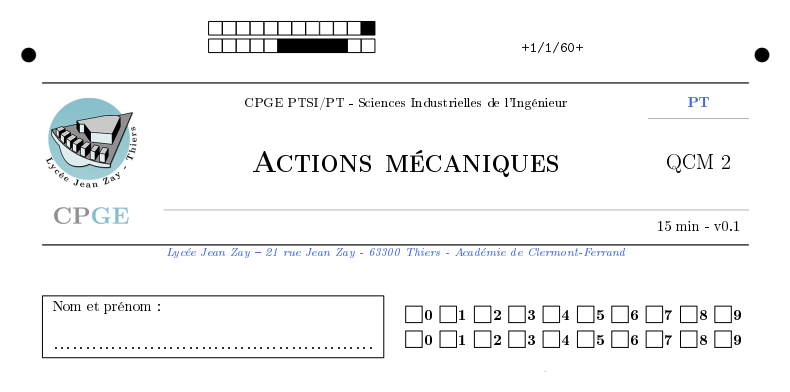
\includegraphics[width=10cm]{Src/Images/defaultQCMHeader.png}}
\end{figure}

\begin{figure}[!ht]
    \centering
	\fbox{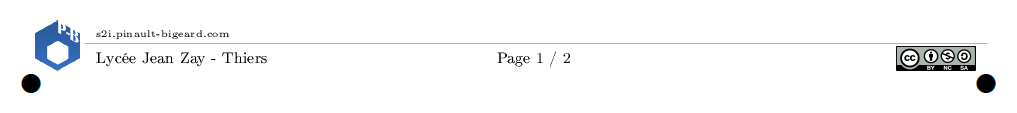
\includegraphics[width=10cm]{Src/Images/defaultQCMFooter.png}}
\end{figure}

\UPSTItitreStd[1]{Commandes spécifiques pour le template QCM}
\begin{itemize}
\item \color{UPSTIcustomColor1}\verb!\UPSTIamcZoneIdentification[opt nbDigits][opt codeChamp]!\color{black}: affiche le champ d'identification de l'étudiant (Nom + code étudiant)
\begin{itemize}
\item \codeBleu{nbDigits}: nombre de chiffres pour le code étudiant (par défaut: 2)
\item \codeBleu{codeChamp}: nom du champ identification pour AMC.
\end{itemize}
\end{itemize}


\subsubsection{Template pour les sujets de colle\label{templateKholle}}
\begin{figure}[!ht]
    \centering
	\fbox{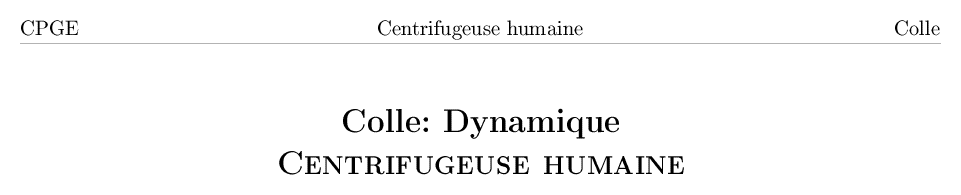
\includegraphics[width=10cm]{Src/Images/defaultKholleHeader.png}}
\end{figure}

\begin{figure}[!ht]
    \centering
	\fbox{
\includegraphics[width=10cm]{Src/Images/defaultKholleFooter.png}}
\end{figure}

\vspace{1em}
\UPSTItitreStd{Paramètres obligatoires:}
\begin{itemize}
\item \codeBleu{UPSTIidVersionDocument}: version prof ou élève (voir \S \ref{profEleve}):
\begin{itemize}
\item \codeBleu{1}: version prof (avec le corrigé affiché);
\item \codeBleu{2}: version élève (sans le corrigé); 
\item \codeBleu{3}: version à publier.
\end{itemize}
\item \codeBleu{UPSTItitreEnTete}: thème du sujet de colle;
\item \codeBleu{UPSTItitre}: titre du sujet de colle;
\item \codeBleu{UPSTInumeroVersion}: version du document.
\end{itemize}

\UPSTItitreStd{Paramètres facultatifs}
\begin{itemize}
\item \codeBleu{UPSTIdocumentCollegial}: si le document est fait par une équipe;
\end{itemize}



\subsection{Style basic\label{styleBasic}}

\subsubsection{Template par défaut}
\begin{figure}[!ht]
    \centering
	\fbox{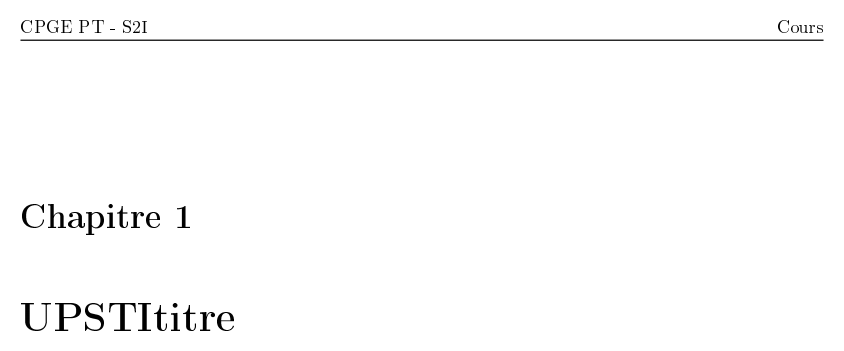
\includegraphics[width=10cm]{Src/Images/basicdefaultHeader.png}}
\end{figure}

\begin{figure}[!ht]
    \centering
	\fbox{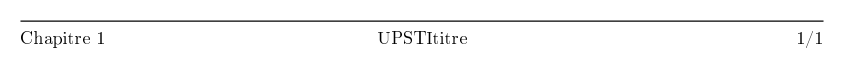
\includegraphics[width=10cm]{Src/Images/basicdefaultFooter.png}}
\end{figure}

\vspace{1em}
\UPSTItitreStd{Paramètres obligatoires}
\begin{itemize}
\item \codeBleu{UPSTIidClasse}: code classe:
\vspace{-1em}
\begin{multicols}{3}
\begin{itemize}
\item \codeBleu{0}: Custom (définir manuellement \UPSTIcode{UPSTIclasse} dans le préambule du document) 
\item \codeBleu{1}: PTSI
\item \codeBleu{2}: PT (défaut)
\item \codeBleu{3}: PCSI
\item \codeBleu{4}: PSI
\item \codeBleu{5}: MPSI
\item \codeBleu{6}: MP
\item \codeBleu{7}: TSI1
\item \codeBleu{8}: TSI2
\item \codeBleu{9}: ATS
\item \codeBleu{10}: PC
\item \codeBleu{11}: Sup
\item \codeBleu{12}: Spé  
\end{itemize}
\end{multicols}
\vspace{-1em}
\item \codeBleu{UPSTIidTypeDocument}: type de document (Cours, TD, TP, etc...):
\vspace{-1em}
\begin{multicols}{3}
\begin{itemize}
\item \codeBleu{0}: Custom (définir manuellement \UPSTIcode{UPSTItypeDocument} dans le préambule du document) 
\item \codeBleu{1}: Cours (défaut) 
\item \codeBleu{2}: TD
\item \codeBleu{3}: TP
\item \codeBleu{4}: Colle
\item \codeBleu{5}: DS
\item \codeBleu{6}: DM
\item \codeBleu{7}: Fiche Méthode
\item \codeBleu{8}: Fiche Synthèse
\item \codeBleu{9}: Formulaire
\item \codeBleu{10}: Mémo
\item \codeBleu{11}: Dossier Technique
\item \codeBleu{12}: Dossier Ressource
\item \codeBleu{13}: Concours Blanc
\item \codeBleu{14}: Document Réponses
\item \codeBleu{15}: Programme de colle
\item \codeBleu{16}: QCM
\end{itemize}
\end{multicols}
\vspace{-1em}
\item \codeBleu{UPSTIidVersionDocument}: version prof ou élève (voir \S \ref{profEleve}):
\begin{itemize}
\item \codeBleu{1}: version prof (avec le corrigé affiché);
\item \codeBleu{2}: version élève (sans le corrigé); 
\item \codeBleu{3}: version à publier.
\end{itemize}
\item \codeBleu{UPSTItitre}: titre principal.
\end{itemize}

\UPSTItitreStd{Paramètres facultatifs}
\begin{itemize}
\item \codeBleu{UPSTIidMatiere}: code matière (S2I, IPT, TIPE...);
\begin{itemize}
\item \codeBleu{0}: Custom (il faut définir manuellement \UPSTIcode{UPSTIintituleMatiere} et \UPSTIcode{UPSTIsigleMatiere};
\item \codeBleu{1}: S2I (défaut);
\item \codeBleu{2}: IPT; 
\item \codeBleu{3}: TIPE.
\end{itemize}
\item \codeBleu{UPSTImessage}: texte personnalisé dans la ligne sous le titre dans le bandeau;
\item \codeBleu{UPSTInumeroChapitre}: numéro du chapitre.
\end{itemize}



\subsubsection{Template pour les QCM AMC}
\begin{figure}[!ht]
    \centering
	\fbox{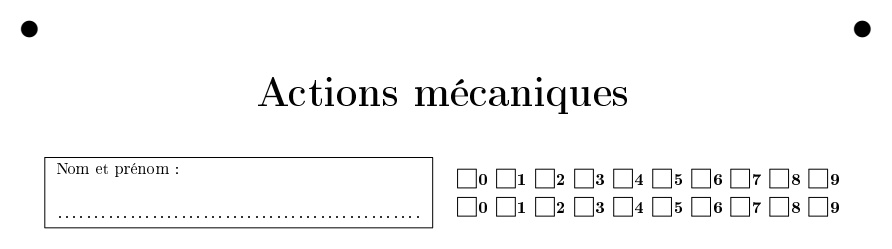
\includegraphics[width=10cm]{Src/Images/basicQCMHeader.png}}
\end{figure}

\begin{figure}[!ht]
    \centering
	\fbox{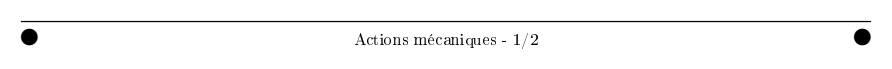
\includegraphics[width=10cm]{Src/Images/basicQCMFooter.png}}
\end{figure}

\UPSTItitreStd[1]{Commandes spécifiques pour le template QCM}
\begin{itemize}
\item \color{UPSTIcustomColor1}\verb!\UPSTIamcZoneIdentification[opt nbDigits][opt codeChamp]!\color{black}: affiche le champ d'identification de l'étudiant (Nom + code étudiant). Voir \S \ref{templateQCM}.
\end{itemize}

\subsubsection{Template pour les sujets de colle\label{templateKhollebasic}}
\begin{figure}[!ht]
    \centering
	\fbox{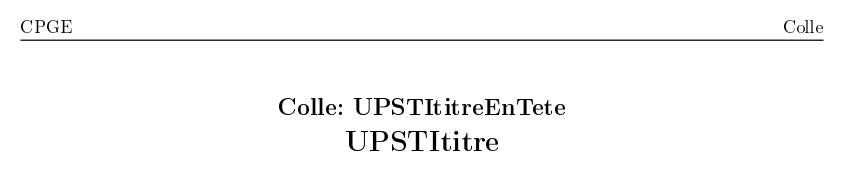
\includegraphics[width=10cm]{Src/Images/basicKholleHeader.png}}
\end{figure}

\begin{figure}[!ht]
    \centering
	\fbox{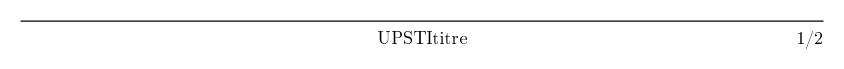
\includegraphics[width=10cm]{Src/Images/basicKholleFooter.png}}
\end{figure}

\vspace{1em}
\UPSTItitreStd{Paramètres obligatoires:}
\begin{itemize}
\item \codeBleu{UPSTIidVersionDocument}: version prof ou élève (voir \S \ref{profEleve}):
\begin{itemize}
\item \codeBleu{1}: version prof (avec le corrigé affiché);
\item \codeBleu{2}: version élève (sans le corrigé); 
\item \codeBleu{3}: version à publier.
\end{itemize}
\item \codeBleu{UPSTItitreEnTete}: thème du sujet de colle;
\item \codeBleu{UPSTItitre}: titre du sujet de colle;
\end{itemize}

\subsection{Style vide\label{styleVide}}
Lorsque l'option \UPSTIcode{vide} est utilisée, les en-têtes et pieds de page sont vides. On peut utiliser cette option si on ne souhaite pas que le package \UPSTIcode{UPSTI\_Document} gère la mise en page.

\subsection{Corrigés UPSTI\label{corrigeUPSTI}}
Ce style est utilisé pour la rédaction de corrigés à utiliser au nom de l'UPSTI. On peut sans problème l'utiliser avec les options \UPSTIcode{noCustomPackages} voire même \UPSTIcode{noPackages}, si on souhaite conserver ses habitudes de rédaction des documents \LaTeX.


% Filière (à classer par ordre alphabétique si nécessaire)
\newcommand{\UPSTIfiliere}{PT}

% Épreuve
\newcommand{\UPSTIepreuveIntitule}{Sciences Industrielles A}
\newcommand{\UPSTIepreuveSigle}{SIA}

% Session
\newcommand{\UPSTIsession}{2017}

% Titre dans l'en-tête
\newcommand{\UPSTItitreSujet}{Manipulateur chirurgical}      

% Auteur (facultatif, n'apparaitra pas sur le corrigé publié)
\renewcommand{\UPSTIauteur}{Prénom NOM}

\UPSTItitreStd[1]{Paramètres obligatoires}
\begin{itemize}
\item \codeBleu{UPSTIidConcours}: code concours:
\vspace{-1em}
\begin{multicols}{2}
\begin{itemize}
\item \codeBleu{0}: Custom (définir manuellement \UPSTIcode{UPSTIconcoursIntitule} et \UPSTIcode{UPSTIconcoursSigle} dans le préambule du document) 
\item \codeBleu{1}: Banque PT
\item \codeBleu{2}: CCMP
\item \codeBleu{3}: CCS
\item \codeBleu{4}: e3a
\item \codeBleu{5}: X/ENS
\item \codeBleu{6}: CCP
\item \codeBleu{7}: ATS
\end{itemize}
\end{multicols}
\vspace{-1em}
\item \codeBleu{UPSTIidVersionDocument}: version prof ou élève (voir \S \ref{profEleve}):
\begin{itemize}
\item \codeBleu{1}: version prof (diffusée sur la partie privée du site de l'UPSTI);
\item \codeBleu{2}: version élève (avec image en filigrane et page d'avertissement). 
\end{itemize}
\item \codeBleu{UPSTIfiliere}: filière concernée (on peut indiquer plusieurs filières ex: MP, PSI, TSI);
\item \codeBleu{UPSTIepreuveIntitule}: intitulé de l'épreuve (ex: Sciences Industrielles A);
\item \codeBleu{UPSTIepreuveSigle}: sigle de l'épreuve (ex: SIA);
\item \codeBleu{UPSTIsession}: année de l'épreuve;
\item \codeBleu{UPSTItitreSujet}: sujet traité.
\end{itemize}

\UPSTItitreStd{Paramètres facultatifs}
\begin{itemize}
\item \codeBleu{UPSTIauteur}: auteur(s) du corrigé.
\end{itemize}

\subsection{Modèle perso\label{modelePerso}}
Si on souhaite utiliser ses modèles de documents personnels, ou si on souhaite modifier les styles distribués par défaut dans le package, on peut modifier le fichier \UPSTIfichier{UPSTI\_Modele\_Perso.sty}.

Il faudra cependant garder la structure de ce fichier et bien évidemment le manipuler avec précaution !


\section{Script de compilation rapide (pour Windows)}
\subsection{Présentation}
Ce package est distribué avec le VBscript \UPSTIfichier{UPSTIcompilRapide.vbs} qui peut être utilisé sous Windows et qui a plusieurs fonctions:
\begin{itemize}
\item permettre la compilation des fichiers \UPSTIfichier{.tex} depuis l'explorateur Windows;
\item créer en une seule manipulation le fichier prof et le fichier élève si nécessaire;
\item zipper automatiquement l'ensemble des fichiers nécessaires à la compilation du document;
\item uploader les fichiers sur un serveur FTP si nécessaire.
\end{itemize}

\UPSTIattention{Ce script n'est absolument pas robuste. Il fonctionne, mais il doit être utilisé avec des pincettes... Mais quand tout fonctionne, le gain de temps est important.}

\subsection{Installation}
\begin{wrapfigure}{r}{4.2cm}
  \centering
  \vspace{-2em}
  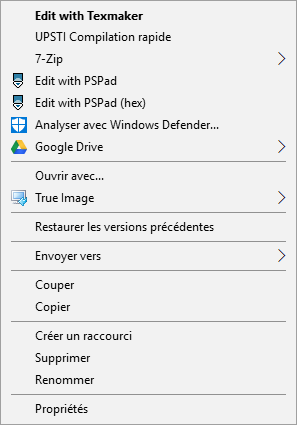
\includegraphics[width=4cm]{Src/Images/menuContextuel.png}
  \vspace{-3em}
\end{wrapfigure}
Il faut dans un premier temps copier le fichier \UPSTIfichier{UPSTIcompilRapide.vbs} dans un dossier sur le disque (ex: \UPSTIfichier{D:\textbackslash LaTeX\textbackslash});

Il faut ensuite éditer le fichier \UPSTIfichier{RegUPSTIcompilRapide.reg} fourni avec le package pour mettre à jour le dossier (s'il est différent de \UPSTIfichier{D:\textbackslash LaTeX\textbackslash}).

Ensuite, on peut double-cliquer sur ce fichier pour ajouter les informations au registre. Dès lors, lorsqu'on fera un clic droit sur un fichier \UPSTIfichier{.tex}, on devrait voir apparaître l'option \UPSTImenuLog{UPSTI Compilation Rapide} dans le menu contextuel (voir ci-contre).

Il faut ensuite installer \UPSTIlogiciel{7zip}: \href{http://www.7-zip.org/}{http://www.7-zip.org/}.

\subsection{Configuration du script}
Il faut éditer le fichier \UPSTIfichier{UPSTIcompilRapide.vbs} avec un éditeur de texte et compléter la section \og Paramètres du script\fg{}.

\subsection{Organisation des dossiers}
\begin{wrapfigure}{r}{4.2cm}
  \centering
  \vspace{-1em}
  \fbox{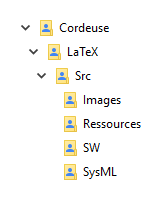
\includegraphics[width=3cm]{Src/Images/dossiers.png}}
  \vspace{-1em}
\end{wrapfigure}
\noindent Pour que le script fonctionne, il faut respecter une certaine organisation des dossiers:
\begin{itemize}
\item \textbf{Niveau 0}: le dossier principal du document (\UPSTIfichier{Cordeuse} dans l'exemple ci-contre). C'est ici que le script va copier les versions compilées du document ainsi que le fichier montrant le numéro de version;
\item \textbf{Niveau 1}: le fichier \UPSTIfichier{.tex} sera stocké dans un sous-dossier \UPSTIfichier{LaTeX} du dossier principal. On y disposera le fichier \UPSTIfichier{@parametres.upsti} qui est un fichier texte qui contient un mot de 6 chiffres:
\begin{itemize}
\item 1\ier{} chiffre: vaut 1 si on doit compiler la version élève. 0 sinon.
\item 2\ieme{} chiffre: vaut 1 si on doit compiler la version prof. 0 sinon.
\item 3\ieme{} chiffre: vaut 1 si on doit uploader un diaporama. 0 sinon.
\item 4\ieme{} chiffre: vaut 1 si on souhaite créer un zip lors de la compilation. 0 sinon.
\item 5\ieme{} chiffre: vaut 1 si on souhaite compiler une version \og À publier\fg{} (voir \S \href{aPublier}). 0 sinon.
\item 6\ieme{} chiffre: vaut 1 si on souhaite que le script copie les fichiers compilés dans le dossier de niveau 0.
\end{itemize}
\end{itemize}

\vspace{-\UPSTIparskipValue}
\begin{itemize}
\item \textbf{Niveau 2}: dans ce dossier, on stockera toutes les fichiers qui seront intégré au zip lors de la compilation (dont les images nécessaires à la compilation. Voir arborescence ci-dessus).
\end{itemize}

\subsection{Upload sur un serveur FTP}
Si on souhaite uploader les documents compilés et les sources sur un serveur FTP, il faut remplir 3 conditions:
\begin{itemize}
\item avoir complété les informations relatives au serveur FTP dans le fichier \UPSTIfichier{UPSTIcompilRapide.vbs};
\item avoir installé \UPSTIlogiciel{ncFTP} (voir dans le zip du package);
\item avoir disposé dans le dossier Niveau 1 un fichier texte \UPSTIfichier{@dossierFTP.upsti} contenant le dossier dans lequel uploader les fichiers sur le serveur FTP.
\end{itemize}

Si le dossier contenant le fichier \UPSTIfichier{.tex} ne contient pas le fichier \UPSTIfichier{@dossierFTP.upsti} alors la phase d'upload est simplement ignorée par le script.

\subsection{Convention de nommage}
Admettons que le fichier \UPSTIfichier{.tex} s'appelle \UPSTIfichier{monFichier.tex}. Le script de compilation créera les fichiers suivants (selon le contenu de \UPSTIfichier{@parametres.upsti}):
\begin{itemize}
\item \UPSTIfichier{monFichier.tex}: version élève ou à publier;
\item \UPSTIfichier{monFichier-Prof.tex}: version prof (corrigé...);
\item \UPSTIfichier{monFichier-Eleve.tex}: s'il s'agit d'un cours (document avec les zones à compléter. Voir \S \href{aPublier}.
\end{itemize}

Si on souhaite uploader aussi un diaporama, celui-ci devra s'appeler: \UPSTIfichier{monFichier-Diaporama.pptx}.

\section{Migration depuis le package EPB\_Cours.sty}
Dans le zip du package, on trouvera aussi un fichier \UPSTIfichier{Migration EPB-UPSTI.py}. En l'exécutant, on peut aller choisir un fichier \UPSTIfichier{.tex} utilisant les packages \UPSTIfichier{EPB\_Cours}, \UPSTIfichier{EPB\_SI} et \UPSTIfichier{EPB\_Pedagogique}. Le script se chargera de l'adapter au package \UPSTIfichier{UPSTI\_Document}.

Là encore, le script n'est pas parfait, mais fonctionnel dans la très grande majorité des cas.

\end{document}
